\chapter{Differentially Private Multi-Party Communication}
In \Cref{ch:dp-shaping}, we explained our differentially private traffic shaping mechanism. 
In this setup, each end-point only communicates with one other end-point at a time. 
Hence, we excluded de-anonymization attacks, which involves adversaries attempting to uncover the fact that two parties are engaged in communication, rather than revealing the content of the communication.
Furthermore, we assumed a one-hop communication in which the adversary monitors the traffic between two middleboxes.
In order to generalize our findings to scenarios involving multi-party communication, we establish two fundamental communication scenarios: 1- One-to-many communication, and 2- Multi-hop communication. 
We illustrate how we can extend DP guarantees to cover one-to-many communication scenarios.
We leave the multi-hop scenario as future avenue of research.


\section{One-to-Many Differentially Private Communication}
We assume an application is communicating with $N$ parties at a time.
We extend the notation proposed in \Cref{sec:dp-shaping-definitions} and represent an application stream as a series of $N$ packet sequences:
\begin{equation}
  \istream = <\istream^1, \istream^2, \dots, \istream^N>
\end{equation}
\noindent
where we have:
\begin{align*}
  \istream^1 &= \{{P^{S^1}_1}, {P^{S^1}_2}, {P^{S^1}_3}, \dots \} \\
  \istream^2 &= \{{P^{S^2}_1}, {P^{S^2}_2}, {P^{S^2}_3}, \dots \} \\
  \vdots& \\
  \istream^N &= \{{P^{S^N}_1}, {P^{S^N}_2}, {P^{S^N}_3}, \dots \} 
\end{align*}
\noindent
where $P^{S^k}_i = (l_i^{S^k}, t_i^{S^k})$ indicates that the $i$\textsuperscript{th} input packet sent to $k$\textsuperscript{th} receiving party in communication has length $l_i$ and transmitted at time $t_i$.
\\
\noindent
We make the assumption that all receiving parties are situated behind distinct middleboxes, thereby leading to $N$ parallel communications. \Cref{fig:one-to-many-communication} visually represents this scenario.
This assumption does not restrict the expendability of this scenario as if more than one receiving parties are placed behind the same middlebox, we can merge their packet sequences into one sequence and reduce the number of parallel communications to $N' < N$.   
\begin{figure}[t]
  \centering
  %  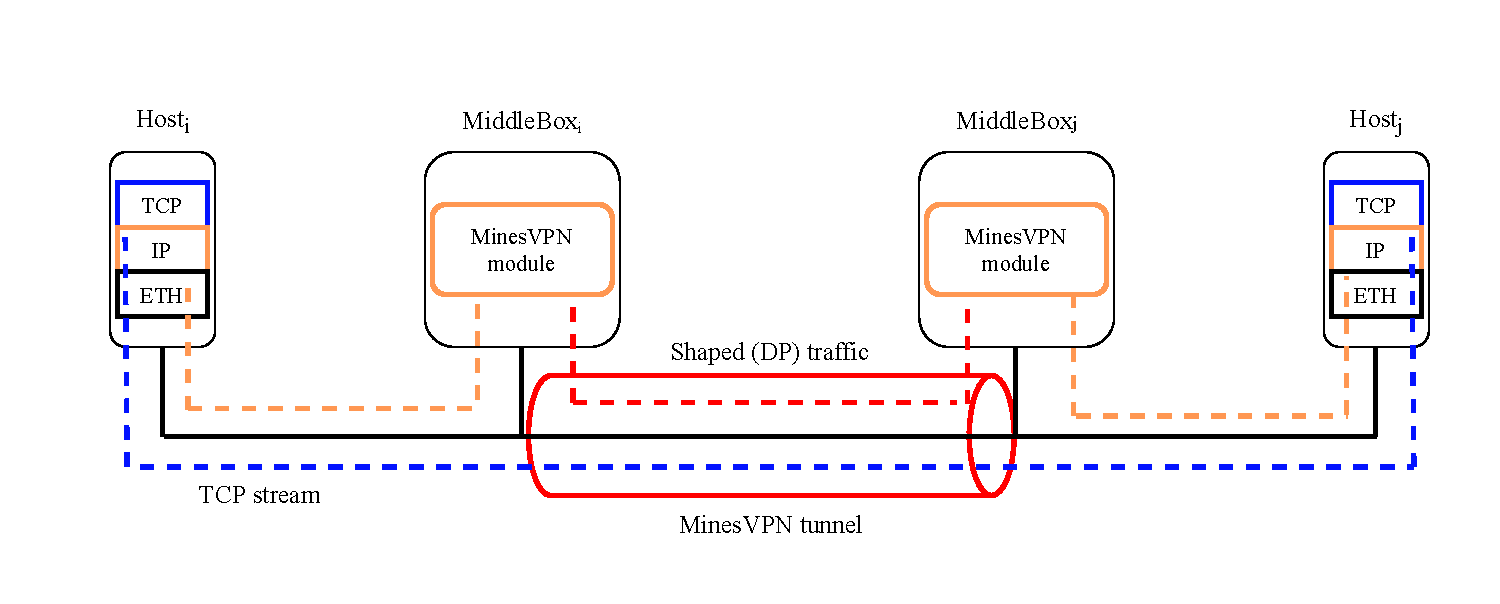
\includegraphics[width=\columnwidth]{figures/Design_highlevel.pdf}
  %  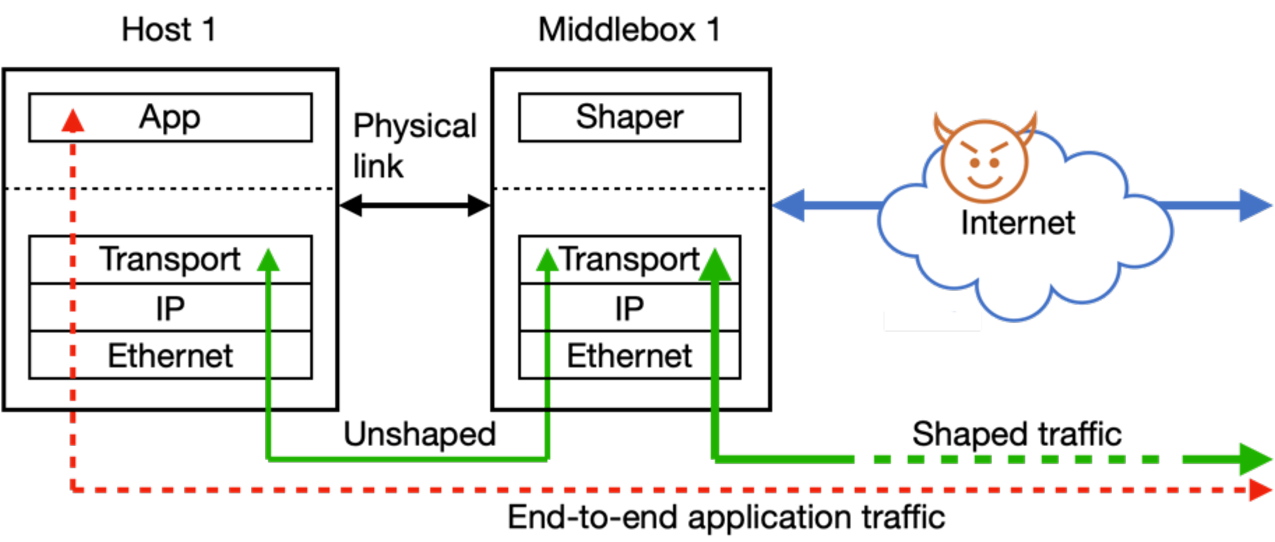
\includegraphics[width=\columnwidth]{figures/minesvpn-overview-half.pdf}
  %  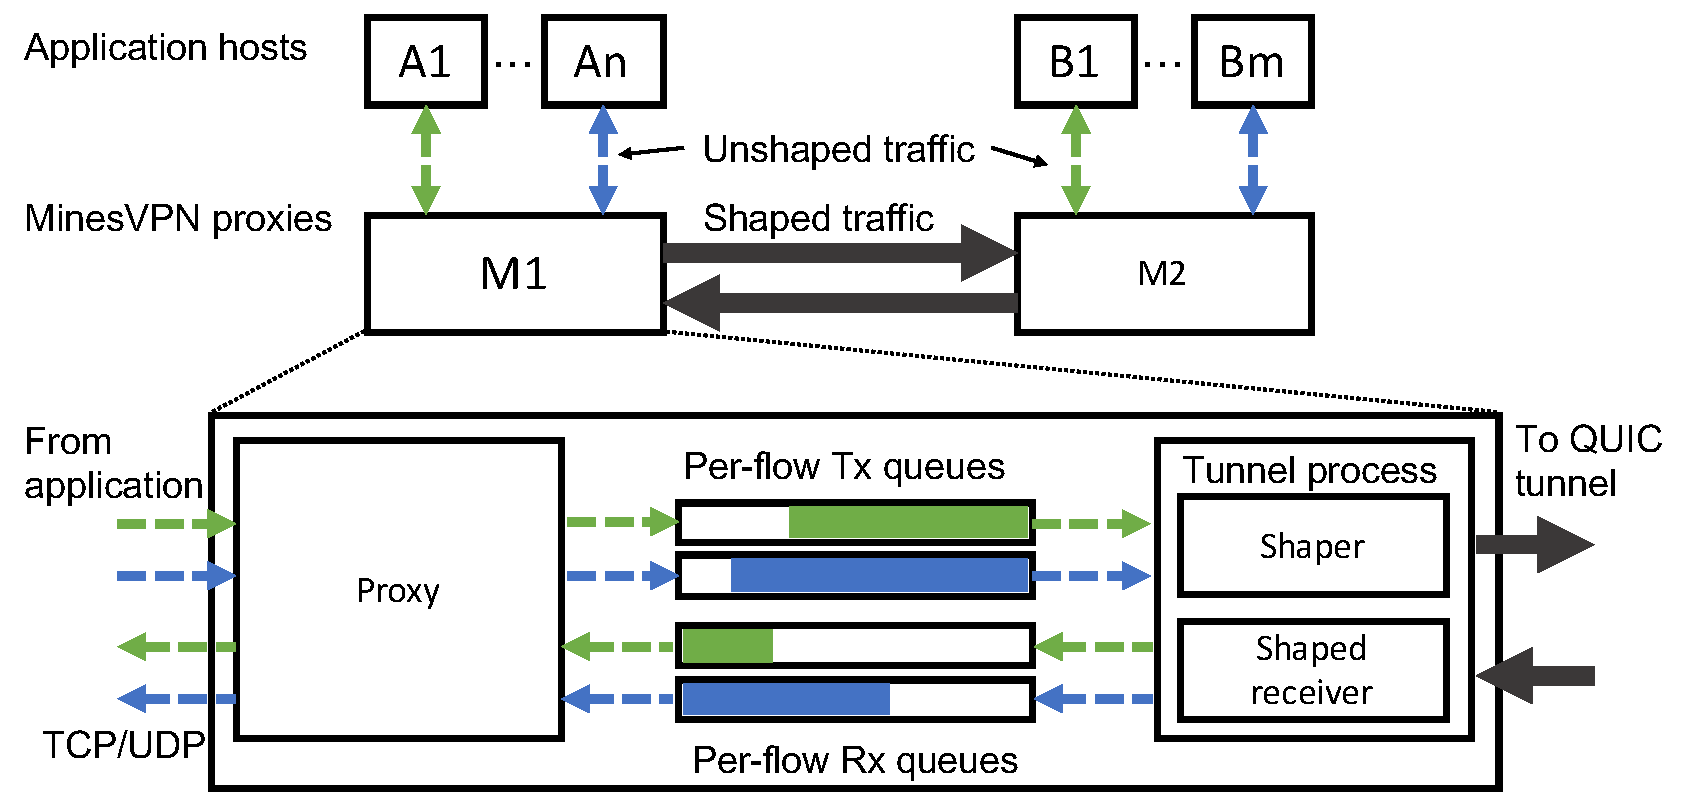
\includegraphics[width=\columnwidth]{figures/minesvpn-arch4.pdf}
  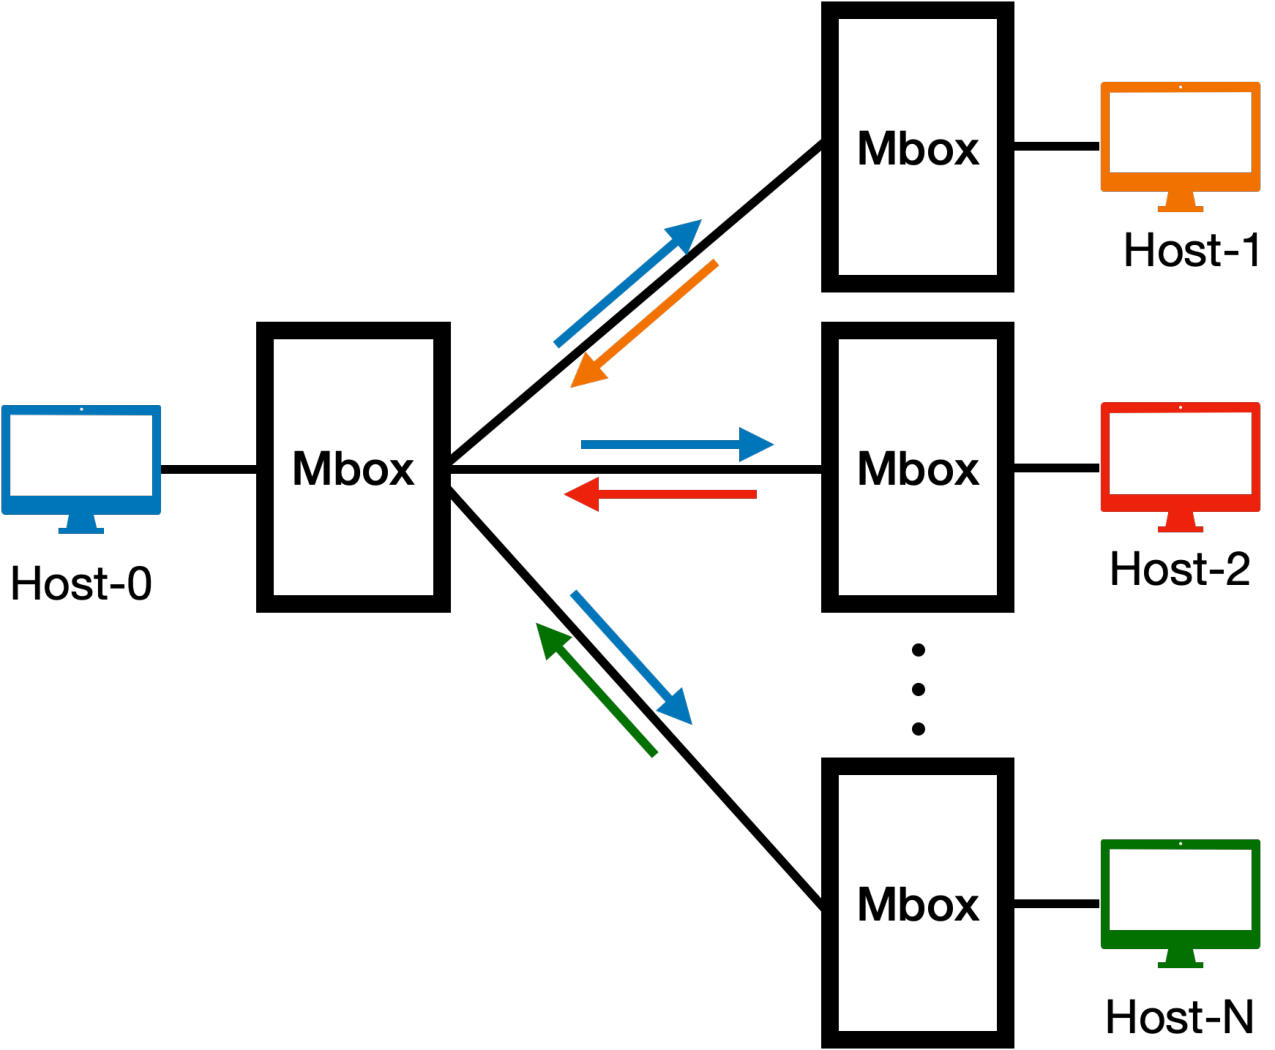
\includegraphics[width=0.7\columnwidth]{figures/one-to-many-communication.pdf}
  \caption{
    One-to-Many parallel communication.
  }
  \label{fig:one-to-many-communication}
\end{figure}



We extend the concept of \textit{buffering queue} that we introduce in \Cref{sec:dp-shaping-definitions} to a \textit{set of $N$ buffering queues} for an application, one for each of pair of communicating parties.  
Each of these queues enqueue the incoming data from application parallel streams with one party within windows of the size of $W$. 
In other words, \Cref{assumption:window} holds true for all $N$ queues simultaneously. 
Similar to \Cref{sec:dp-shaping-definitions}, we define a set of stream subsequences over a window $j$ and represent it with $\istream_j = <\istream^1_j, \istream^2_j, \dots, \istream^N_j>$, such that $k \in [N]:~\istream_j^k = \{P^{\istream^k}_i | P^{\istream^k}_i \in \istream^k~and~t_i^{S^k} \in j\}$. 
Intuitively, a set of stream subsequences is a slice with a length $W$ across all parallel communications with $N$ parties.
We re-define the \Cref{def:neighboring-streams} to match the new setup.
\begin{definition}[Neighboring Series of Streams]\label{def:neighboring-series-stream}
  Two sets of $N$ stream subsequences $S_{j}$ and $\hat{S}_{j}$ transmitted in a window $j$ are neighbors if the L1-norm distance between all corresponding subsequences is at most~$\ssens$ bytes in a window of up to length $\winlen$.
  \\
  In other words: 
  \begin{equation*}
    \forall k \in [n]: {\norm{~S_{j}^k - \hat{S}_{j}^k~}}_1 \leq \ssens
  \end{equation*}
\end{definition}
\noindent
For each subsequence, we define the sensitivity value of its dedicated queue over the intervals of length $T$. 
We represent the sensitivity of a subsequence $S_{j}^k$ with $\qsens^k$: 
\begin{equation}
  \qsens^k = \max_{l = 0}^{\numupdates}~\max_{\streamw{j}^k,
      \hat{\streamw{j}^k}} | \qlent{l}^k - \hat{\qlent{l}^k} |
  \label{eqn:ssens-multi-stream}
\end{equation}
where $\qlent{l}^k$ and  $\hat{\qlent{l}^k}$ are queue lengths of the subsequence $S_{j}^k$ and subsequence $\hat{S_{j}^k}$ at the beginning of the $l$\textsuperscript{th} interval respectively.
The shaping mechanism is independently applied to each packet subsequence, $S_{j}^k$, at intervals of $T$ based on its sensitivity, $\qsens^k$, as we explained in \Cref{subsec:dp-shaping-mechanism}.
Therefore, each queue measurement is $(\varepsilon_T, \delta_T)$-DP.
The transmitted packet sequence is denoted as $N$ sequences of packets observable by adversary:
\begin{equation}
  \ostream = <\ostream^1, \ostream^2, \dots, \ostream^N>
\end{equation}
\noindent 
where we have:
\begin{align*}
  \ostream^1 &= \{{P^{O^1}_1}, {P^{O^1}_2}, {P^{O^1}_3}, \dots \} \\
  \ostream^2 &= \{{P^{O^2}_1}, {P^{O^2}_2}, {P^{O^2}_3}, \dots \} \\
  \vdots& \\
  \ostream^N &= \{{P^{O^N}_1}, {P^{O^N}_2}, {P^{O^N}_3}, \dots \} 
\end{align*} 
We assume that the adversary's goal is to expose the contents of a single packet sequence, $\ostream^k$.
In pursuit of this objective, the adversary strategically exploits the information made available through other packet sequences.
To calculate the privacy loss of measuring all queues for all stream subsequences at each interval, we need to differentiate between two different communication setup: Independent subsequences and Correlated subsequences.   

To measure dependency between stream subsequence, we use the correlation between two streams such that for an application stream with $N$ series of packet sequences $\istream = <\istream^1, \istream^2, \dots, \istream^N>$, we have:
\begin{equation*}
  \forall i,j \in [N]:~Corr(\istream^i, \istream^j) = c_{ij}
\end{equation*}
\noindent
This enables us to define a correlation matrix $C$ such that $[C]_{ij}=c_{ij}$.
We assume the correlation coefficients to have the following properties:
\begin{enumerate}
  \item For all $i,j \in [N]$, $-1 \leq c_{ij} \leq 1$, with $-1$ representing that two subsequences are negatively correlated (\ie when one exists in the stream the other one does not and vice versa), $1$ representing that they are fully correlated (\ie they appear in the stream always together), and $0$ means no correlation.
  \item For all $i \in [N]$, $c_{ii} = 1$.
\end{enumerate}
Various correlation metrics fulfill the aforementioned conditions, with the Pearson correlation coefficient~\cite{cohen2009pearson} being the most prevalent among them. 
\noindent
Calculating privacy loss for independent sequences (\ie $\forall i \neq j \in [N]:~corr(\istream^i, \istream^j) = 0$) is straightforward. 
In independent communication setup, monitoring one sequence does not reveal any information about others. 
Therefore, each stream subsequence is $(\varepsilon_T, \delta_T)$-differentially private.
Nonetheless, in a correlated setup, the adversary has the ability to monitor a single packet sequence, thereby acquiring preceding information about others, which consequently results in further privacy breaches. 
In the following section, we present a systematic approach for quantifying privacy loss in interdependent packet subsequences.
















% \subsection{One-to-Many Independent Communication}
% In this regime of communication, We assume an application is communicating with $N$ parties independently.
% If we represent an application stream with $N$ series of packet sequences $\istream = <\istream^1, \istream^2, \dots, \istream^N>$, all packet sequences are mutually uncorrelated:
% \begin{equation*}
%   \forall i \neq j \in [N]:~corr(\istream^i, \istream^j) = 0
% \end{equation*}
% \noindent
% This assumption is particularly correct for message passing and video streaming applications as these applications provide service for non-related entities.
% For this setup, we argue that the privacy loss of measuring all subsequence queues with DP is the same as privacy loss associated with each individual queue.
% \begin{proposition}\label{prop:independent-subsequence}
%   Assume all packet sequences within an application stream are mutually uncorrelated, if we measure each subsequence queue size with $(\varepsilon_T, \delta_T)$-DP with a sensitivity of $\qsens^k$, measuring queue sizes for all subsequences is also $(\varepsilon_T, \delta_T)$-DP.  
% \end{proposition} 
% \begin{proof}
%   (informal) As packet subsequences are independent, releasing a DP measurement of a queue for one subsequence does not affect the adversary's prior knowledge regarding any other subsequences. 
%   Therefore, the privacy loss associated with the communication between a single pair does not change. 
% \end{proof}
% \noindent
% Based on \Cref{prop:independent-subsequence}, we can measure the privacy loss of a 1-to-$N$ communication simply by extending results of \Cref{prop:dp} to a multiparty communication as follows:
% \begin{proposition}\label{prop:independent-stream-privacy}
%   In the one-to-many independent communication setup, {$\sys$} enforces $(\varepsilon_{\winlen}, \delta_{\winlen})$-DP for each pair of communicating entities within the window of length $W$, with $\varepsilon_{\winlen}, \delta_{\winlen} \triangleq
%   \textrm{DP\_compose}(\varepsilon_T, \delta_T, \numupdates)$.
% \end{proposition}


\subsection{One-to-Many Correlated Communication}
In many applications,  simultaneous communications with distinct entities are interdependent.
For example, many businesses use online advertising platforms such as Google Ads to create and run ads on various websites.
Therefore, every time a user requests the website, the web browser retrieves content from both the web server hosting the website and the online advertising platform that hosts the website's Ads.   
This is, in fact, an example of a one-to-many correlated communication setup.
\\
In standard definition of differential privacy, we assume data points to be independent.  
However, measuring the privacy loss when entries of database are correlated is challenging.
We consider this problem from two related, yet different, perspectives. 



\subsubsection{Correlated Communication, Correlated Sensitivity}
One approach to ensure DP guarantees for a correlated communication involves adjusting the sensitivity of each packet sequence to account for the correlation that might reveal extra information.
Intuitively, the correlation between packet sequences can amplify the impact of altering a single sequence, extending its influence beyond its designated buffering queue and subsequently influencing the queue size for other sequences.
For instance, in the running example of online advertising platforms, removing the request to the targeted website not only changes the queue size buffering the website data but also affects the size of the queue storing data from advertising servers.

Quantifying the impact of the dependency between packet sequences is difficult. 
First, it demands extensive monitoring of the relationships between sequences to accurately measure their effects.
Secondly,  in the absence of well-defined assumptions regarding the structure of packet sequences, formulating a correlation metric capable of encapsulating this interdependency poses a considerable challenge.
To tackle this issue, one strategy is to assume that for any pair of correlated packet sequences, they exhibit complete correlation
Then, for any packet subsequence $\istream^k_j$, scale its sensitivity with the number of packet subsequences that have correlation with it.
Therefore, if we represent the adjusted correlated sensitivity of packet sequences $\istream^k_j$ with $(\qsens^k)_{corr}$, we have:
\begin{equation}\label{equ:naive-correlated-sensitivity}
  (\qsens^k)_{corr} = n^k.\qsens^k 
\end{equation}
\noindent where $n^k$ is the number of packet subsequences that are correlated with $\istream^k_j$.
\\
This implies a consistent co-occurrence of these two packet sequences within the application stream (\eg the website consistently loading ads alongside its content).
Chen\etalc{chen2014correlated} prove this approach to be differentially private.
Scaling the sensitivity by the number of correlated packet sequences diminishes utility, as we treat even slightly correlated sequences as fully correlated.
To improve the utility of this approach, Zhu\etalc{zhu2014correlated} propose a new definition for correlated sensitivity that accounts for the \textit{correlation degree} of data points. 
They further assume that data points in a database to be linearly related.  
Following the method of Zhu~\etal, we define correlated sensitivity for each packet sequence:
\begin{definition}[Correlated Sensitivity]\label{def:correlated-sensitivity} 
  For each packet subsequence $S_{j}^k$, we define the correlated sensitivity value of its dedicated queue over the interval of length of $T$, and calculate it as follows:
  \begin{equation}\label{equ:correlated-sensitivity}
    (\qsens^k)_{corr} = \sum_{m=0}^{N} |c_{mk}|. \big( \max_{l = 0}^{\numupdates}~\max_{\streamw{j}^m,
    \hat{\streamw{j}^m}} | \qlent{l}^k - \hat{\qlent{l}^k} | \big) 
  \end{equation}
\end{definition}
\noindent where $c_{mk}$ captures the \textit{correlation degree} between packet sequence $\istream^m_j$ and $\istream^k_j$. 
Intuitively, the correlated sensitivity for a packet sequence captures the effect of adding/removing all other packet sequences on a designated sequence, $\istream^k_j$.
From \Cref{def:correlated-sensitivity}, it is clear that:
\begin{equation}
  \qsens^k \leq (\qsens^k)_{corr} \leq n^k.\qsens^k
\end{equation} 
\noindent where $n^k$ is the number of packet subsequences that are correlated with $\istream^k_j$.
This implies that using \Cref{def:correlated-sensitivity} improves the utility of DP shaping mechanism.
Nonetheless, the limitation of this approach resides in its assumption of linear interrelation among packet sequences, implying that the queue size for one packet sequence can be expressed as a linear function of the others.
Many applications might violate this assumption, leading to a higher-than-expected privacy loss.




\subsubsection{Correlated Communication, Composition Theorem}
We can interpret results of \Cref{equ:naive-correlated-sensitivity} through the lens of the Differential Privacy (DP) composition property (refer to \Cref{subsubsec:background-dp-composition}).
The complete correlation between two packet subsequences indicates their consistent co-occurrence. 
Therefore, in the context of the "website request" event, the DP shaping mechanism performs two DP measurements: one DP measurement of the queue storing website data and another measurement of the queue that contains Ads data.
This simultaneous release of result from a differentially private mechanism exemplifies the self-composition property of DP, and the privacy loss associated with it can be quantified using different variants of composition theorem (\Cref{prop:basic-composition}, \Cref{prop:advanced-composition}, and \Cref{prop:rdp-composition}).
In fact, \Cref{equ:naive-correlated-sensitivity} is a representation of basic composition theorem (\Cref{prop:basic-composition}). 
To explain this, we consider a simple Laplace mechanism in which, according to the \Cref{def:laplace-mechanism}, the additive noise to the queue length of a packet sequence $\istream^k$ has a distribution of $Lap(\qsens^k/\varepsilon)$.
If we adjust the sensitivity to account for correlation (\ie $(\qsens^k)_{corr} = n^k.\qsens^k$) while preserving the same distribution of the additive noise, the adjusted privacy loss is $\varepsilon_{corr} = n^k \varepsilon$.
This manifests the results of basic composition theorem.

Quantifying the privacy loss of correlated communication using DP composition property has two main advantages: 
First, it enables us to employ refined adaptations of composition theorems, such as R\'enyi composition~\cite{mironov2017renyi}, to measure the privacy loss associated with our shaping mechanism.
Secondly, with composition theorem, we can also quantify the privacy loss of correlated packet sequences in case that each packet subsequence is shaped with different privacy parameters ($\varepsilon, \delta)$.
However, a limitation of this approach is that, in contrast to the correlated sensitivity outlined in \Cref{def:correlated-sensitivity}, the composition theorem assumes complete correlation among packet sequences.
Neither of these approaches have a consistent superiority over the other one, and privacy-utility trade-offs of them might change based on the underlying pattern of database.
